\chapter{Overview of the tool Storm}\label{storm-chapter}

Storm \cite{storm1} is a probabilistic model checker implemented in \verb|C++| recently released. It is able to analyse
four Markov models, featuring discrete-time Markov chains and Markov decision processes. The main aim of this tool is to be competitive in terms of performance, to be updated with new verification algorithms, to be able to
deal with a large panel of modelling languages,... This tool provides %many other
a lot of model checking features, including solvers for all the problems presented in the previous chapters, including multi-objective problems.
In this chapter, we present how MDPs can be defined in this powerful tool, how they are represented and with which different approaches problems are solved.

\section{Models}
As mentioned above, Storm allows to model-check four types of Markov models.
The first family of models is discrete-time Markov models, that are covered in the first chapter, composed by
discrete-time Markov chains and Markov decision processes.
The second family of models is continuous-time Markov models, composed by continuous-time Markov chains and Markov automata. \\

Continuous-time Markov chains (CTMC, for short) \cite{maro} are similar to discrete-time Markov chains, but each state $s$ is
characterised by an exit rate $\lambda_s$.
The time $t$ spent in each state $s$ of the system is negatively exponentially distributed with this rate, i.e., the probability to stay in $s$ after $t$ time units passed in $s$ is $e^{- \lambda_s t}$.
This exit rate and a probability transition function allow to induce a generator
function with which it is possible to compute the probability
%to go from one state to another after a certain time.
that the system is currently in a state $s'$ while the system was in the state $s$, $t$ time units ago.
Note that the ``step'' notion is replaced by the ``time'' notion in comparison with discrete-time models. Furthermore, a Markov automaton (MA, for short) is a continuous-time nondeterministic Markov model where the key idea is the same as between MCs and MDPs in discrete-time. \\

We will not dwell on continuous-time models anymore and focus primarily on discrete-time models.

\section{Input formats}
Storm supports various native input formats, including Prism, Jani, generalised stochastic Petri nets, dynamic fault trees, cpGCL and explicit format.
We will introduce the three input languages supported by the main executable of Storm by presenting how to use them to model our
discrete-time systems.
\subsection{Prism} \label{prism-subsec}
The Prism language \cite{prismsynt} allows to deal with MCs, CTMCs and MDPs in Storm.
It is a state-based language using reactive \textit{modules}.
We will not define the complete syntax and semantic of the Prism language, but rather provide a way to
define our MDPs.
Let $\mathcal{M} = (S, A, \Delta, w, AP, L)$ be a finite MDP, with $|S| = n$, and $s_i \in S$ be the $i^{\text{th}}$ state of $S$.
In Prism, this state $s_i$ corresponds to the initial state of the system. That is, the probability measure that we consider is defined on paths starting from $s_i$.\\

In the Prism language, a \textit{module} represents a component of the system.
By definition of our MDPs, we just need a single module to
represent them. A module allows to characterise $S$, $A$ and $\Delta$. We begin by enumerating states of $\mathcal{M}$:
\[
  x: [0\, ..\, n-1] \; \text{init} \; i;
\]
In the Prism language, $x$ is considered as a \textit{variable} of the module, ranging over states of $\mathcal{M}$.
In this manner, we express that for all $j \in \{0, \dots, n-1\}$, $s_j \in S$
is the $j^{\text{th}}$ state of $S$ represented by the index $j$ of the variable $x$ (i.e., $x=j$), and $s_i$ is the initial state from which events start, represented by the index $i$ of the variable $x$ (i.e., $x=i$).
Note that a variable represents a set of states of the MDP. Thus, it is possible that a module has more than one variable if the state space of the MDP is formed by a Cartesian product of set of states.
Thanks to variables of the module, it is possible to form predicates $\Phi$ on the variables of the module with the syntax described with the following grammar:
\begin{align*}
  \Phi &::= true \; \mid \; x \varphi p \; \mid \; (X) \; \mid \; (\mathcal{E}) \\
  X &::= \Phi \; \mid \; \Phi \& X \\
  \mathcal{E} &::= \Phi \; \mid \; \Phi | \mathcal{E}
\end{align*}
where $x$ is a variable of the module, $\varphi \in \{<, \leq, >, \geq, =, \neq\}$
and $p \in \mathbb{N}$. Let $s \in S$ be a state of $\mathcal{M}$. We have that $s \models \Phi$ iff $\Phi$ is true for the state $s$, i.e.,
\begin{itemize}
  \item $s \models true$,
  \item $s \models x \varphi p$ iff there exists an index $j \in \mathbb{N}$ in the range of indices of the module variable $x$ by which the state $s$ is represented (i.e., $s$ is represented by $x=j$) and such that $j \varphi p$.
  \item $s \models (\Phi_1 \& \dots \& \Phi_m)$ iff
    for all $k \in \{1, \dots, m\}$, $s \models \Phi_k$, and
  \item $s \models (\Phi_1 | \dots | \Phi_m)$ iff
    there exists $k \in \{1, \dots, m\}$ such that $s \models \Phi_k$.
\end{itemize}
We denote by $Sat(\Phi)$ the set of states satisfying the predicate $\Phi$, i.e., $Sat(\Phi) = \{s \in S \; | \; s \models \Phi\}$.

\begin{example}[\textit{Satisfaction of a predicate on variables of an MDP module}] Consider an MDP $\mathcal{M}$ with state space $S$ and a Prism program containing a module $M$ defining this MDP.
Assume that the size of the state space $S$ is $|S| = 5$ and that the module $M$ contains a unique variable $x$, ranging over all states of $S$. Let
$\Phi = (x \leq 1 \,||\, x >3)$ be a predicate on the variables of the module $M$, then $Sat(\Phi) = \{s_0, s_1, s_4\}$.
\end{example}

The behaviours of the module, i.e., transitions of the set $\rightarrow$\footnote{Remind that the transition relation $\rightarrow$ is the set $\{ (s, \alpha, s') \in S \times A \times S \; | \; \Delta(s, \alpha, s') > 0 \}$} are then described
inside the module by a set of \textit{guarded commands}, taking the following form:
\[
  [\alpha] \; \Phi \rightarrow \delta_1: \phi_1 + \dots + \delta_m: \phi_m;
\]
where $\Phi$ is a predicate over the variables of the module such that, for all $s \in Sat(\Phi)$, $\alpha \in A(s)$, $i \in \{1, \dots, m\}$, $\delta_i \in [0, 1]$ with $\sum_{i=1}^m \delta_i = 1$ and where $\phi_i$ is an \textit{update formula} describing a state represented by a variable of the module. This guarded command basically means that all states that satisfy the predicate $\Phi$ go to the state  described by $\phi_i$ with a probability $\delta_i$, when the action $\alpha$ is chosen.
An update formula $\phi$ is of the form
\[\phi::=(x'_1=u_1) \& (x'_2=u_2) \& \dots \& (x'_k=u_k)\]
where $x_1, x_2, \dots, x_k$ are variables of the module and $u_1, u_2, \dots, u_k$ are \textit{expressions} (i.e., literal values, variables, constants and operators) over all variables.
% \begin{align*}
%   \phi &::= (s'=\chi) \; | \; (s'= \mu(\chi, \chi)) \; | \; \psi \\
%   \chi &::= s \varphi x \; | \; x \\
%   \psi &::= \phi \; | \; \phi \& \psi
% \end{align*}
% where $s$ is a variable of the module,
% $\varphi \in \{+, -\}$, $\mu \in \{\min, \max \}$ and $x \in \mathbb{N}$.
% Let assume that the system is currently in the $j^\text{th}$ state of $S$, i.e.,
% in the state $s_j$
% %The expression $\chi$ actually represents the core of a variable update ; it represents the index of the state to which the system evolves.
% %\begin{itemize}
% %  \item $\chi = x$ directly refers to the index $x$ of the variable to update and
% %  \item $\chi = s \varphi x$ refers to the current index of the variable $s$ on which the operation $\varphi x$ is applied (here, $j \varphi x$).
% %\end{itemize}
% and let $k \in \{0, \dots, n-1\}$. We have that $s_k \models \phi$ iff $\phi$ refers to the state $s_k$, i.e.,
% \begin{itemize}
%   \item $s_k \models s' = x$ iff $k = x$. Then the system go from $s_j$ to $s_x$.
%   \item $s_k \models s' = s \varphi x$ iff $k$ is the current index of the variable $s$ on which the operation $\varphi$ has been applied. Here, we have $k = j \varphi x$. Thus the system go from $s_j$ to $s_{j+\varphi}$.
% \end{itemize}
\begin{example}[\textit{Guarded command for a simple module}]
Let $\mathcal{M} = (S, A, \Delta, w, AP, L)$ be an MDP. Consider that all states of $\mathcal{M}$ are represented by the values of the single variable $x$, ranging on all states of the set $S$, with $|S|=n$, the transitions of $\mathcal{M}$ can be described with the following guarded command:
let $s_j$ be the $j^{\text{th}}$ state of $S$, for all enabled actions $\alpha \in A(s_j)$ of $s_j$,
\[
  [\alpha] \; x=j \rightarrow \delta_0: x'=j_0 + \dots + \delta_{m-1}:  x'=j_{m-1};
\]
where $s_{j_0}, \dots, s_{j_{m-1}}$ are $\alpha$-successors of $s_j$ and $\delta_k = \Delta(s_j, \alpha, s_{j_k})$,
with  $m=|Succ(s_j,\alpha)|$, $k \in \{0, \dots, m-1\}$, $j_k \in \{0, \dots, n-1\}$ and where $s_{j_k}$ is the $k^\text{th}$ $\alpha$-successor of $s_j$ and the $j_k^\text{th}$ state of $S$.
\end{example}

The set of atomic propositions $AP$ and the labelling function $L$ of $\mathcal{M}$ are characterised in the Prism language as follows: for all $a \in AP$,
\[
  \text{label} \; ``a" = \Phi;
\]
where the set of states satisfying the predicate $\Phi$ is actually the set of states labelled with $a$, i.e., $Sat(\Phi) = \{ s \in S \; | \; a \in L(s) \}$. \\

% \[
%   \text{label} \; ``a" = (s=j_0\, \& \, \dots \, \& \, s=j_{m-1});
% \]
% where $S_a= \{s \in S \; | \; a \in L(s) \}$ and $s_{j_k} \in S_a$,
% with $m = |S_a|$, $k \in \{0, \dots, m-1\}$,
% $j_k \in \{ 0, \dots, n-1 \}$ and $s_{j_k}$, the $k^\text{th}$ state of $S_a$ and the $j_k^\text{th}$ state of $S$.
%

Finally, the weight function $w$ can be characterised with the notion of \textit{rewards}. In the Prism language, it is possible to associate to each transition
of the set %$\{ (s, \alpha, s') \in S \times A \times S \; | \; \Delta(s, \alpha, s') > 0 \}$
$\rightarrow$
a real value. A \textit{dimension rewards} is a set of rewards taking the following form:
\[
  [\alpha] \; \Phi: x;
\]
where $\alpha \in A$ is an action, $\Phi$ is a predicate and $x \in \mathbb{R}$
is the value of the reward of going from a state $s \in S$, such that $\alpha \in A(s)$, to states of $Sat(\Phi)$. Note that if the action $\alpha$ is omitted (giving a reward of the form $[]\; \Phi: x^*;$), each transition $s \xrightarrow{\,\alpha\,} s'$ such that $s' \in Sat(\Phi)$ and $\alpha \in A(s)$
has a reward of $x^*$. Note also that it is possible to specify multiple dimensions rewards, allowing to define multi-dimensional MDPs.
We can adapt the reward notion to describe the weight function of our MDPs with a set of rewards formed as follows:
let $\alpha \in A$ be an action of $\mathcal{M}$ and $x = w(\alpha)$, the reward formed by
\[
  [\alpha] \; true: x;
\]
is actually the weight of the action $\alpha$.

\begin{example}[\textit{Defining an MDP in the Prism language}]
Let $\mathcal{M}=(S, A, \Delta, w, AP, L)$ be the MDP of Figure \ref{prism-simple}. This MDP can be defined in the Prism language as follows:
\begin{figure}[h!]
\begin{minipage}{0.4\linewidth}
  \lstinputlisting[language={Prism},
      rulesepcolor=\color{black}, rulecolor=\color{black},
      breaklines=true,
      breakatwhitespace=true, firstnumber=1, firstline=1, lastline=25]{resources/simple_mdp.prism}
\end{minipage}
\begin{minipage}{0.6\linewidth}
    \includegraphics[width=\linewidth]{resources/simple-mdp}
\end{minipage}
\captionsetup{justification=centering}
\caption{MDP $\mathcal{M}$, with $S = \{s_0, s_1, s_2\}$, $A = \{\alpha, \beta, \gamma\}$ and $AP = \{a, b\}$}\label{prism-simple}
\end{figure}
\end{example}

\begin{example}[\textit{Unfolding of an MDP in the Prism language}]
Let $\mathcal{M}$ be the MDP of Figure \ref{prism-simple} with state space $S$ and $\ell \in \mathbb{N}$
be a length threshold such that $\ell=8$. We can define the unfolding of $\mathcal{M}$ from the state $s_0$ until the length threshold $\ell$ for the set of target states $T = \{s_1\}$ (cf. Figure \ref{unfolding}) in the Prism language as follows:
\lstinputlisting[language={Prism},
    rulesepcolor=\color{black}, rulecolor=\color{black}, breaklines=true,
    breakatwhitespace=true, firstnumber=1, firstline=1, lastline=25]{resources/unfolded_simple_mdp.prism}
\end{example}
Since the state space of the unfolded MDP $\mathcal{M}_\ell$ is a Cartesian product between the state space $S$ of $\mathcal{M}$ and the set $V = \{0, \dots, \ell, \bot\} \subseteq \mathbb{N} \cup \{\bot\}$, we can define the variables of the unfolded MDP $\mathcal{M}_\ell$ with the variables of $\mathcal{M}$ and a new variable $v$, ranging from $0$ to $\ell+1$ (where the $(\ell+1)^\text{th}$ state actually represents the $\bot$ value). The guarded
commands of the module are obviously defined, following the definition of the
probability transition function $\Delta_\ell$ of any unfolded MDP. Finally, a label $target$ is added,
labelling each state of the set $T_\ell = \{ (t, v) \in S \times V \; | \; t \in T \; \wedge \; v \leq \ell \}$.

\subsection{Explicit format}
Storm also supports input models specified in explicit format. The syntactic power of such a format is lower compared to the Prism language, but is
very simple and intuitive.
%Thereby, this format can thus be interesting in case of
%we want to verify a model generated from another tool (e.g., MRMC or Prism).
%In general, a same model generated in explicit format from different tool does not match exactly. However, it can be easily modified by hand to be handled by Storm due to
%the simplicity of the format.
Moreover, this format has the advantage of being supported by several model checkers.\\

An MDP specified in explicit format
consists of a transition matrix file, describing explicitly transitions of the system, a reward matrix file, describing explicitly
rewards of these transitions, and a labelling set file. More formally, let $\mathcal{M} = (S, A, \Delta, w, AP, L)$ be an MDP.
We assume the state space $S$ is enumerated as $S = \{0, \dots, n-1\}$ and the set of enabled action $A(s)$ is enumerated as $A(s) = \{0, \dots, m-1\}$, for all $s \in S$.
%, where $|S| = n$ and where $A(s)$ is countable for all $s \in S$.
The transition matrix $P$ and the reward matrix $R$ of sizes $(|\rightarrow|, 4)$ are defined as follows.
% let $l \in \{1, \dots, |\rightarrow|\}$ be the $l^\text{th}$ line of $P$ and $R$,
% \begin{itemize}
%   \item $P_{l, 1} = R_{l, 1}$ is the index $i$ of the source state $s_i \in S$ of the $l^\text{th}$ transition of $\rightarrow$,
%   \item $P_{l, 2} = R_{l, 2}$ is the index $k$ of an enabled action of $s_i$ in $A(s_i)$,
%   \item $P_{l, 3} = R_{l, 3}$ is the index $j$ of the target state $s_j \in S$ of this transition and
%   \item $P_{l, 4}$ is the nonzero transition probability $p$ given by $\Delta(s_i, \alpha_{s_i, k}, s_j)$, where $\alpha_{s_i, k}$ denotes the $k^\text{th}$ enabled action of $A(s_i)$.
%   \item $R_{l, 4}$ is the reward of the transition $(s_i, \alpha_{s_i, k}, s_j)$.
% \end{itemize}
% Thus, the line $l \in \{1, \dots, |\rightarrow|\}$ of $P$ defined by the vector $(i, k, j, p) \in \mathbb{N}^3
% \times [0, 1]$ describes that the state $s_i$ goes to the state $s_j$ by choosing
% the $k^\text{th}$ enabled action $\alpha_{s_i, k}$ of $A(s_i)$ with a probability $p = \Delta(s_i, \alpha_{s_i, k}, s_j)$. In a similar way,
% the line $l' \in \{1, \dots, |\rightarrow|\}$ of $R$ defined by the vector
% $(i, k, j, r) \in \mathbb{N}^3 \times \mathbb{R}$ describes that the state $s_i$ goes to the state $s_j$ by choosing the $k^\text{th}$ enabled action $\alpha_{s_i, k}$ of $A(s_i)$ with a reward $r$.
% Since rewards of our MDPs are actually costs of actions, this reward $r$ equals $w(\alpha_{s_i, k})$. \\
Let $(s, \alpha, s')$ be the $l^\text{th}$
transition of $\rightarrow$, we have $P_{l, 1} =
R_{l, 1} = s$, $P_{l, 2} = R_{l,2} = \alpha$,
$P_{l,3} = R_{l,3} = s'$, and $P_{l, 4} = \Delta(s, \alpha, s')$ and $R_{l, 4} = w(\alpha)$.
Additionally, labels of this MDP are described with a set of vectors $Lab$ defined as follows : \[Lab = \{(s, a_1, \dots, a_k) \in \mathbb{N} \times AP^k \; | \; k = |L(s)| \wedge \{a_1, \dots, a_k\} = L(s)\}.\]
Note that if $L(s)= \emptyset$ for a given state of the system, this state can be omitted in $Lab$.

\begin{example}[\textit{Define an MDP in explicit format}]
Let $\mathcal{M}$ be the MDP of Figure \ref{prism-simple}. The explicit transition matrix $P$, the explicit reward matrix $R$ and the explicit set of labels $Lab$ of $\mathcal{M}$ are defined as follows:
  \begin{equation*}
  P =
  	\begin{pmatrix}
  	0 & 0 & 1 & \frac{1}{2} \\[0.3em]
  	0 & 0 & 2 & \frac{1}{2} \\[0.3em]
  	1 & 0 & 0 & 1 \\[0.3em]
    2 & 0 & 2 & 1 \\[0.3em]
    2 & 1 & 0 & 1
  	\end{pmatrix}, \quad \quad
  R =
    \begin{pmatrix}
  	0 & 0 & 1 & 3 \\[0.3em]
  	0 & 0 & 2 & 3 \\[0.3em]
  	1 & 0 & 0 & 2 \\[0.3em]
    2 & 0 & 2 & 5 \\[0.3em]
    2 & 1 & 0 & 2
    \end{pmatrix}, \quad \quad
  Lab = \{ (0, a), (1, b) \}
  \end{equation*}
For instance, the first transition is explained as follows: the state $s_0$ go to $s_1$ with a probability $\frac{1}{2}$, choosing its first enabled action, and the cost of this transition is $3$.
Moreover, the state $s_0$ is labelled with $a$.
Note that the enumeration of actions do not corresponds to the enumeration of the set $A$, but rather the enumeration of the set of enabled action $A(s)$ of each state $s$.
\end{example}

\subsection{Jani}
Jani \cite{JQM} is a recent modeling language whose syntax is based on Json and whose design is based on networks of communicating automata.
The purpose of this language is to provide a stable and uniform interface
between tools and, more particularly, model checkers.
This format supports MCs, CTMCs, MDPs and MAs. \\

The semantic model of the Prism language forms the conceptual basis of
Jani and is extended to also support MAs.
Furthermore, Jani is designed
to be easy to generate and parse programmatically without library dependencies.
However, Jani has not been designed to be created manually by users, but rather
to be automatically generated from higher-level and domain-specific languages, while remaining human-readable, in contrast to binary encodings. Storm actually allows to
convert multiple input types to Jani. An example of conversion in available in Appendix \ref{prism2jani}.


%\section{Implementation}
\section{Engines}
Storm is decomposed in five engines that pursue different approaches to solve a problem.
\begin{itemize}
  \item \textit{Sparse}: this engine is the default one. It uses sparse matrices as in-memory representation of models. Numerical analysis methods allow efficient memory allocation and fast operations for this data structure on small and moderately sized models.
  Actually, this data structure is very powerful where most states of the model have transitions to a small subset of the set of states of the model. This situation actually represents most of the cases: in general, underlying graphs of Markov models are rarely complete and the transition matrix representing the probability transition function of
  most of the models is thus sparse.
  \item \textit{DD}: this engine uses multi-terminal binary decision diagrams (MTBDDs) \cite{Fujita:1997:MBD:607541.607565} as their primal representation. This data structure allows
  to handle gigantic models. Intuitively, each state of the system are encoded on $n$ bits and the probability transition function is a boolean function
  over the bits representation of two states. Binary decision diagrams (BDDs) \cite{PMC} are
  used to represent boolean functions and are actually compressed binary decision trees through directed acyclic graphs (DAGs), with two terminal states ($1$ and $0$). MTBDDs are BDDs allowing numerical values for terminal states.
  \item \textit{Hybrid}: this engine uses MTBDDs as representation of models, but sometimes uses sparse matrices if operations are judged more appropriate with this format.
  \item \textit{Abstraction refinement}: this engine \textit{abstracts} (non-necessary finite) discrete-time Markov models to finite \textit{stochastic games} and automatically \textit{refines} the \textit{abstraction} as necessary. This engine is suited for models with an infinite state space (other engines cannot handle this type of models).
  \par Intuitively, the abstraction consists of constructing a smaller model by removing details from the concrete system.
  The motivation is that when a property hold in the abstract model, then it also holds in the concrete system.
  If the property does not hold in the abstraction, then either information from the model checking process allows to exhibit a counter-example to show that the property is false in the concrete system, or the abstraction is refined.
  \par Constructing an abstraction of an MDP implies a greater degree of nondeterminism.
  The process of abstraction must maintain a distinction between the nondeterminism from the original MDP and from the nondeterminism induced during the abstraction process, and this is why stochastic games are used \cite{DBLP:journals/fmsd/KattenbeltKNP10}.
  \item \textit{Exploration}: this engine uses sparse representation for models and explores the state space of models with machine learning methods.
\end{itemize}

\section{Solvers}
Several solvers are available in Storm.
Storm uses the suited solver according to the situation (i.e., the input model, its format, the engine used and its in-memory representation).

\begin{itemize}
  \item \textit{Linear equation systems}: Storm provides a
    solver for linear equation systems, allowing to handle reachability and expectation properties in MCs.
  \item \textit{Bellman equations}: these equations form
    systems defined in the next chapter for MDPs (cf. Theorem
    \ref{bellman1} and Appendix \ref{bellman2}) whose solutions describe
    reachability and expectation properties.
    The associated solver is based on an approximation technique named \textit{value iteration} (cf. Subsection \ref{temp-event-mdp}).
    Intuitively, this technique approximates values of the solution of the equation by iteratively updating the approximation. This approximation is guaranteed to converge to the solution of the equation system.
    Therefore, the difficulty of this technique is to find a threshold used to stop the iteration process.
    \par Since numerical methods are prone to numerical problems, Storm supports enabling \textit{exact arithmetic} to obtain precise results.
  \item \textit{Linear programming}: a solver for (mixed-integer) linear programs is implemented in Storm, allowing to describe reachability and expectation properties for MDPs.\par
  If the size of the considered MDP is sufficiently moderate, Storm uses this solver as the primary.
  \item \textit{SMT}: an SMT problem is a decision problem for first-order logical formulae with equality and without quantifier. SMT solvers are used to minimise the size of models by \textit{bisimulation}.
  A bisimulation is an equivalence relation between two systems having the same behaviour.
  \item \textit{Stochastic games}: although Storm does not support stochastic games as input format,
    solvers for them are available for the abstraction refinement engine
    which uses these as representation.
  \item \textit{Multi-objective}: this solver allows to compute $\epsilon$-approximations of Pareto curves (cf. Subsection \ref{le-pareto} and Section \ref{mo-mc}), for a given $\epsilon > 0$.
\end{itemize}

\section{Model checking}
Storm properties are expressed in a language including PRCTL and CSL (i.e., \textit{continuous stochastic logic}, for continuous Markov models).
The syntax of the subset of this language supporting PRCTL is slightly different than the classical PRCTL, and we present in this section the slight changes in comparison to the classical PRCTL syntax presented in Chapter \ref{model-checking-chapter}. We denote by \textit{Storm-PRCTL} the subset of the Storm language supporting PRCTL.

\begin{notation}[\textit{MC and MDP support by the syntax of Storm-PRCTL}]
  Let $\mathcal{M}$ be an MDP. In this section, we cover at a time the syntax of Storm-PRCTL for MCs and MDPs.
  As a reminder, we can consider an MC as an MDP such that there is only one enabled action for each state.
  The differences between PRCTL for MCs and for MDPs are probabilistic operator and expected operator.
  %,
  %referring to the probability and the expected cost-to-target in the MC context, and referring to the maximum probability and the minimum expected cost-to-target in the MDP context.
  Indeed, in the context of MCs, these operators are $\mathcal{P}_J(\phi)$ and $\mathcal{E}_C(\Phi)$, referring to the probability of an event formed by a path formula $\phi$ and the expected cost-to-target of the satisfaction set of a state formula $\Phi$.
  In the context of MDPs, these operators are $\mathcal{P}^{\max}_J(\phi)$ and $\mathcal{E}^{\min}_C(\Phi)$, referring to the maximum probability of an event formed by a path formula $\phi$ and the minimal expected cost-to-target of the satisfaction set of a state formula $\Phi$.
  So, let the words
  \[\lambda = \begin{dcases*}
    \varnothing &if $\mathcal{M}$ is an MC\\
    \max & else
  \end{dcases*} \;\text{ and }\;
  \mu = \begin{dcases*}
    \varnothing &if  $\mathcal{M}$ is an MC\\
    \min & else
  \end{dcases*}\]
  where $\varnothing$ is the empty word.
  We can now generalise the syntax of these operators with $\mathcal{P}^\lambda_J(.)$ and $\mathcal{E}^\mu_C(.)$ according to $\mathcal{M}$ in PRCTL and we use this notation for the syntax of Storm-PRCTL.
\end{notation}

\begin{definition}[\textbf{Syntax of Storm-PRCTL}]
Let $\mathcal{M}$ be an MDP with space of atomic proposition $AP$,
\begin{itemize}
  \item Storm-PRCTL \textit{state formulae} over $AP$ are formed according to the following grammar:
  \[ \mathsf{
    \Phi ::= true \;\; | \;\;} ``a" \;\; | \;\;\mathsf{
    \Phi_1 \, \& \, \Phi_2 \;\; | \;\; ! \Phi \;\; |
    \;\; P\lambda\,{\varphi}}\,j \mathsf{ \, [\phi] \;\; |
    \;\; R\mu\,{\varphi}\,}c \mathsf{ \,[F\, \Phi]
    }
  \]
  where $a \in AP$ is an atomic proposition, $\phi$
  is a path formula, $\varphi \in \{=, <, >, \leq,
  \geq \}$, $ j \in [0, 1]$, and $c
  \in \mathbb{N} \cup \{+\infty\}$.
  \item Storm-PRCTL \textit{path formulae} over $AP$ are formed according to the following grammar:
  \[\mathsf{
    \phi ::= X \Phi \;\; | \;\; \Phi_1 \, U \, \Phi_2
    \;\; | \;\; \Phi_1 \, U\leq }\,n\mathsf{ \, \Phi_2
    \;\; | \;\; \Phi_1 \, U\{ ``d" \}\leq \ell \, \Phi_2
  }
  \]

  where $\mathsf \Phi$, $\mathsf \Phi_1$ and
  $\mathsf \Phi_2$ are state formulae, $\mathsf d$ is a \textit{dimension reward} (cf. Subsection \ref{prism-subsec}), and $n, \ell \in \mathbb{N}$.
\end{itemize}
\end{definition}

% \begin{definition}[\textbf{Translation of Storm-PRCTL into PRCTL}]
%   Let $\mathcal{M} = (S, A, \Delta, w, AP, L)$ be an MDP, we can \textit{translate} each Storm-PRCTL formula into a classical PRCTL formula with the following functions:
%   \[
%     t_{state}: \text{Storm-PRCTL state formula over }AP \rightarrow \text{PRCTL state formula over }AP,
%   \]
%   \[
%     t_{state}(\Phi) = \begin{cases}
%
%     \end{cases}
%   \]
%
% \end{definition}

\begin{definition}[\textbf{Equivalence between Storm-PRCTL formulae and PRCTL formulae}]
Let $\mathcal{M} = (S, A, \Delta, w, AP, L)$ be an MDP, $\Phi, \, \Psi$ be PRCTL state formulae over $AP$, and $\mathsf{\Phi}, \mathsf{\Psi}$ be Storm-PRCTL state formulae over $AP$,
there is an equivalence relation $\equiv$ over Storm-PRCTL and classical PRCTL state formulae:
\begin{align*}
  \mathsf{true} &\equiv true, & ``a" &\equiv a,  \\
  \mathsf{\Phi \, \& \, \Psi} &\equiv \Phi \wedge \Psi, & \mathsf{!\, \Phi} &\equiv \neg \Phi, \\
  \mathsf{P}{\lambda} \, \varphi\, j \, [\phi] &\equiv \mathcal{P}^{\lambda}_{ \varphi j}(\phi),&
  \mathsf{R}{\mu}\,\varphi \, c \, [\mathsf{F \Phi}] &\equiv \mathcal{E}^{\mu}_{ \varphi c } (\Phi),\\[0.3em]
  \noalign{\centering if and only if $\mathsf{\Phi} \equiv \Phi \text{ and } \mathsf{\Psi} \equiv \Psi,$}
  \intertext{where $a \in AP$, $j \in [0, 1]$, $c \in \mathbb{N}\cup \{+ \infty\}$, and $\phi$ is a PRCTL path formula over $AP$. Additionally, $\mathsf{\Phi \,|\, \Psi} \equiv \Phi \vee
  \Psi \equiv \neg (\neg \Phi \wedge \neg
  \Psi)$ if and only if $\mathsf{\Phi} \equiv \Phi \text{ and } \mathsf{\Psi} \equiv \Psi$. Then, there also exists an equivalence between Storm-PRCTL path formulae and classical PRCTL path formulae:}
  \mathsf{X \Phi} &\equiv \bigcirc \Phi, & \mathsf{\Phi \, U \, \Psi} &\equiv \Phi \U \Psi,\\
  \mathsf{\Phi\, U \leq} n \, \mathsf{\Psi}, &\equiv \Phi \U^{\leq n}\, \Psi, &
  \mathsf{\Phi\, U\{ ``d" \}\leq \ell} \, \mathsf{\Psi} &\equiv \Phi \U_{\leq \ell}\, \Psi,\\[0.3em]
  \noalign{\centering if and only if $\mathsf{\Phi} \equiv \Phi \text{ and } \mathsf{\Psi} \equiv \Psi,$}
  \intertext{where $n, \ell \in \mathbb{N}$ and $\mathsf d$ is a dimension reward. Additionally,}
  \mathsf{F \Phi} &\equiv \Diamond \Phi, \text{ and} & \mathsf{G \Phi} &\equiv \Box \Phi,\\[0.3em]
  \noalign{\centering if and only if $\mathsf{\Phi} \equiv \Phi$.}
\end{align*}
\vspace{-3.5em}
\end{definition}
The semantic of Storm-PRCTL is the same as the semantic of PRCTL following this equivalence between formulae.
Optimised model checking algorithms are implemented in Storm and the main engine supports all properties formed with this syntax.

\begin{example}[\textit{\SSPE{} problem in Storm}]
Let $\mathcal{M}$ be the MDP of Figure \ref{prism-simple}.
We are interested to solve the following \SSPE{} problem:
\[
  ?\exists \sigma \quad \mathbb{E}_{s_0}^\sigma(\TS^{\{s_1\}}) \leq 10,
\]
and we can actually solve this problem by verifying that the following PRCTL property holds in $s_0$:
\[
  \mathcal{E}_{\leq 10}^{\min}(b).
\]
This property is equivalent to the following in Storm-PRCTL:
\[
  \mathsf{Rmin\,\leq 10\, [F \,} ``b"].
\]

We consider the initial states of the Prism program as being the states that we want to verify that properties hold in it.
As we have specified in the Prism program that the initial state is $s_0$, then Storm will model check the input property for this state (cf. Figure \ref{storm-program-2}).

\begin{figure}[h!]
{\footnotesize
\begin{verbatim}
>> storm --prism simple_mdp.prism --prop "Rmin<=10 [F \"b\"]"

Storm 1.2.0

--------------------------------------------------------------
Model type: 	MDP (sparse)
States: 	3
Transitions: 	5
Choices: 	4
Reward Models:  weights
State Labels: 	3 labels
   * deadlock -> 0 item(s)
   * init -> 1 item(s)
   * b -> 1 item(s)
Choice Labels: 	none
--------------------------------------------------------------

Model checking property R[exp]min<=10 [F "b"] ...
Result (for initial states): true

Time for model checking: 0.008s.
\end{verbatim}
}
\captionsetup{justification=centering}
\caption{Verifying that $\mathcal{E}_{\leq 10}^{\min}(b)$ holds in the state $s_0$ of the MDP in Figure \ref{prism-simple} in Storm}
\label{storm-program-2}
\end{figure}
\noindent First, we see that Storm builds the MDP following the input Prism model with the sparse representation. It informs us that the system has five transitions and four nondeterministic choices. Thus, we see that the default dimension reward considered by Storm for this system is the one named \textit{weights} in the program, that is actually the only one in this system.
It also informs us that the system has no deadlock, one initial state (here $s_0$) and one state labelled with $b$ (here $s_1$).
Finally, Storm gives us the result of the model checking by answering \textit{true} to the satisfiability of the property by the state $s_0$.
\end{example}
\begin{example}[\textit{\SSPP{} problem in Storm}]
Let $\mathcal{M}$ be the MDP of Figure \ref{prism-simple}. We are interested to solve the following \SSPP{} problem:
\[
  ? \exists \sigma \quad \mathbb{P}_{s_0}^\sigma(\Diamond_{\leq 8}\, \{s_1\}) \geq \frac{7}{10},
\]
and we can actually solve this problem by verifying that the following PRCTL property holds in $s_0$:
\[
  \mathcal{P}^{\max}_{\geq \frac{7}{10}}(\Diamond_{\leq 8}\, b).
\]
This property is equivalent to the following one in Storm-PRCTL:
\[
  \mathsf{P{max}\geq 0.7 \, [F\{``weights"\}\leq 8 \, }``b"].
\]

As in the previous example, running Storm with the Prism program modelling $\mathcal{M}$ as input with this Storm-PRCTL property allows to verify that this property holds in $s_0$ (cf. Figure \ref{storm-program-1}).% and this is done with the following command line:
\begin{figure}[H]
{\footnotesize
\begin{verbatim}
storm --prism simple_mdp.prism --prop "Pmax>=0.7 [F{\"weights\"}<= 8 \"b\"]"
Storm 1.2.0

--------------------------------------------------------------
Model type: 	MDP (sparse)
States: 	3
Transitions: 	5
Choices: 	4
Reward Models:  weights
State Labels: 	3 labels
   * init -> 1 item(s)
   * deadlock -> 0 item(s)
   * b -> 1 item(s)
Choice Labels: 	none
--------------------------------------------------------------

Model checking property Pmax>=7/10 [true Urew{"weights"}<=8 "b"] ...
Result (for initial states): true

Time for model checking: 0.009s.
\end{verbatim}
\captionsetup{justification=centering}
\caption{Verifying that $\mathcal{P}^{\max}_{\geq \frac{7}{10}}$ holds in the state $s_0$ of the MDP in Figure \ref{prism-simple} in Storm}
\label{storm-program-1}
}
\end{figure}
\noindent Storm confirms that this property holds in $s_0$.
\end{example}

Additionally, Storm allows to formulate probabilistic and expectation queries by replacing the probabilistic and expectation operators by $\mathsf{P\lambda=?[.]}$ and $\mathsf{R\mu=?[.]}$.

\begin{definition}[\textbf{Syntax of Storm-PRCTL queries}]
Let $\mathcal{M}$ be an MDP with state space $S$ and atomic proposition space $AP$, Storm-PRCTL queries over $AP$ are formed according to the following grammar:
\[
  \mathsf{\Phi^? ::= P\lambda=?\,[\phi] \; \; | \; \; R\mu=?\,[F\,\Phi]}
\]
where $\mathsf{\Phi}$ is a Storm-PRCTL state formula and $\phi$ is a Storm-PRCTL path formula.
\end{definition}

\begin{definition}[\textbf{Semantic of Storm-PRCTL queries}]
 Let $\mathcal{M}$ be an MDP with state space $S$ and atomic proposition space $AP$, $s \in S$, $\Phi$ be a Storm-PRCTL state formula over $AP$ and $\phi$ be a Storm-PRCTL path formula over $AP$, the semantic of Storm-PRCTL queries over $AP$ is defined as follows:
 \begin{itemize}
%  \item $P\lambda=? \, [\phi] = (x_s)_{s \in S_0}$ such that $x_s = \mathbb{P}^\lambda_s(\{ \pi \in Paths(s) \; | \; \pi \models \phi \})$, where $s \in S_0$.
%  \item $R\mu=? \, [F\,\Phi] = (x_s)_{s \in S_0}$ such that $x_s = \mathbb{E}^\mu_s(\TS^{Sat(\Phi)})$, where $s \in S_0$.
   \item $\mathsf{P\lambda=? \, [\phi]} = \mathbb{P}^\lambda_s(\{ \pi \in Paths(s) \; | \; \pi \models \phi \})$.
   \item $\mathsf{R\mu=? \, [F\,\Phi]} = \mathbb{E}^\mu_s(\TS^{Sat(\Phi)})$.
 \end{itemize}
\end{definition}
\begin{example}[\textit{Storm-PRCTL query}]
  Let $\mathcal{M}$ be the MDP of Figure \ref{cost-bounded-until5} with atomic proposition space $AP$.
  \begin{figure}[h]
  \centering
  \includegraphics[width=0.7\linewidth]{resources/MDPExample}
  \lstinputlisting[language={Prism},
      rulesepcolor=\color{black}, rulecolor=\color{black},
      breaklines=true,
      breakatwhitespace=true, firstnumber=1, firstline=1]{resources/mdp3.prism}
  \captionsetup{justification=centering}
  \caption{MDP $\mathcal{M}$ from Example \ref{cost-bounded-example}, with state space $S=\{s_0, s_1, s_2, s_3, s_4, s_5, s_5\}$ and with space of atomic propositions $AP = \{a, b, c\}$}
  \label{cost-bounded-until5}
  \end{figure}
  We have shown in Example \ref{cost-bounded-example} that $s_0 \models \mathcal{P}^{\max}_{\geq \frac{1}{5}}((a \vee b) \U_{\leq 8} \, c)$, and we are interested by the maximum probability with which this property holds in $s_0$. Since $s_0$ is the initial state of the Prism program, we can formulate the following Storm-PRCTL query over $AP$ for the state $s_0$:
  \[
    \mathsf{Pmax =? \, ((}``a" \, | \, ``b"\mathsf{) \; U\{``weights"\}<= 8 \;} ``c").
  \]
  We run Storm by passing the Prism program modelling $\mathcal{M}$ as input with this property (cf. Figure \ref{storm-program-3})
\begin{figure}[h!]
  {\footnotesize
% Model type: 	MDP (sparse)
% States: 	6
% Transitions: 	12
% Choices: 	7
% Reward Models:  weights
% State Labels: 	5 labels
%    * init -> 1 item(s)
%    * deadlock -> 0 item(s)
%    * b -> 1 item(s)
%    * c -> 1 item(s)
%    * a -> 1 item(s)
% Choice Labels: 	none
% --------------------------------------------------------------
%
  \begin{verbatim}
Model checking property Pmax=? [("a" | "b") Urew{"weights"}<=8 "c"] ...
Result (for initial states): 0.3325
Time for model checking: 0.000s.
\end{verbatim}
  }
  \captionsetup{justification=centering}
  \caption{Storm-PCRTL query for the MDP in Figure \ref{cost-bounded-until5}}
  \label{storm-program-3}
\end{figure}
Storm informs us that the result of this query is $0.3325$, that corresponds to the solution of the LP defined to verify that the property hold in $s_0$ in Example \ref{cost-bounded-example}.
\end{example}

\section{Multi-objective model checking}\label{mo-mc}

Storm supports multi-objective model checking for MDPs, and allows us to formulate properties extending the Storm-PRCTL language in order to solve multi-objective problems encountered in Chapter \ref{multi-objective-chapter}.

\begin{definition}[\textbf{Syntax of multi-objective Storm-PRCTL}]
  Let $\mathcal{M}$ be an MDP with state space $S$ and atomic proposition space $AP$, and $n \in \mathbb{N}$ Storm-PRCTL state formulae over $AP$ $\mathsf\Phi_i$,
  \textit{multi-objective Storm-PRCTL formulae} over $AP$ are formed according to the following grammar:
  \[
    \mathsf{multi(\Phi_1,\, \dots,\, \Phi_n)}.
  \]
\end{definition}

\begin{definition}[\textbf{Syntax of multi-objective Storm-PRCTL queries}]
  Let $\mathcal{M}$ be an MDP with state space $S$ and atomic proposition space $AP$, $k \in \mathbb{N}_0$ Storm-PRCTL state queries over $AP$
  $\mathsf\Phi_i^?$ for $i \in \{1, \dots, k\}$, and $l$ Storm-PRCTL state formulae over $AP$
  $\mathsf{\Psi_j}$ for $j \in \{1, \dots, l\}$,
  \textit{multi-objective Storm-PRCTL queries} over $AP$ are formed according to the following grammar:
  \[
    \mathsf{multi(\Phi^?_1,\, \dots,\, \Phi^?_k, \Psi_1, \dots, \Psi_l)}.
  \]
\end{definition}

\begin{definition}[\textbf{Achievable points of a multi-objective Storm-PRCTL query}]
Let $\mathcal{M}$ be an MDP with state space $S$ and set of atomic proposition $AP$, $s \in S$, and $\mathcal{Q}$ be a multi-objective Storm-PRCTL query over $AP$ for the state $s$.
This query is composed by $k \in \mathbb{N}_0$ queries of the form $\mathsf{Pmax=?}(\phi_i)$ and $l \in \mathbb{N}$
state formulae of the form $\mathsf{Pmax}(\phi_{k + j})\geq \alpha_i$, where $\alpha_j \in [0, 1]\cap\mathbb{Q}$, $\phi_i$, $\phi_k+j$ are Storm-PRCTL path formulae over $AP$ for $i \in \{1, \dots, k\}, \, j \in \{1, \dots, l\}$.
  The set of achievable points $U_\mathcal{Q}$ is given by
  \begin{align*}
    U_\mathcal{Q} = \{\, p \in [0, 1]^{k+l} \; | \; \exists \sigma, \, \sigma', \, \forall i \in \{1, \dots, k\} \, \forall j \in \{1, \dots, l\},\\
    \mathbb{P}_s^\sigma(Paths(s, \phi_i)) = p_i \; \wedge \; p_j = \mathbb{P}_s^{\sigma'}(Paths(s, \phi_{k+j})) \geq \alpha_j \, \},
  \end{align*}
  where $Paths(s, \phi) = \{ \pi \in Paths(s) \; | \; \pi \models \phi\}$, for a given path formula $\phi$.
\end{definition}

In order to verify multi-objective reachability properties, the multi-objective solver build an approximation of the Pareto curve for the $n$ properties and return \textit{safe} points of the Pareto curve, i.e., points contained in the under-approximation of the Pareto curve, following an approximation value $\epsilon > 0$.
The default approximation technique used to build this Pareto curve is an adaptation of the one presented in \cite{DBLP:journals/corr/abs-1206-6295}.%based on the value-iteration method, %but an adaptation of the constraint based method (like in \cite{DBLP:conf/focs/PapadimitriouY00}) is also implemented.

\begin{example}[\textit{\SSPWE{} problem in Storm}]
  Getting back to Example \ref{sspwe-example}, let $\mathcal{M}$ be the MDP of Figure \ref{sensornet}.
  \begin{figure}[h!]
  \begin{minipage}{0.45\linewidth}
  \lstinputlisting[language={Prism},
      rulesepcolor=\color{black}, rulecolor=\color{black}, breaklines=true,
      breakatwhitespace=true]{resources/sensors.prism}
  \end{minipage}
  \begin{minipage}{0.55\linewidth}
    \centering
    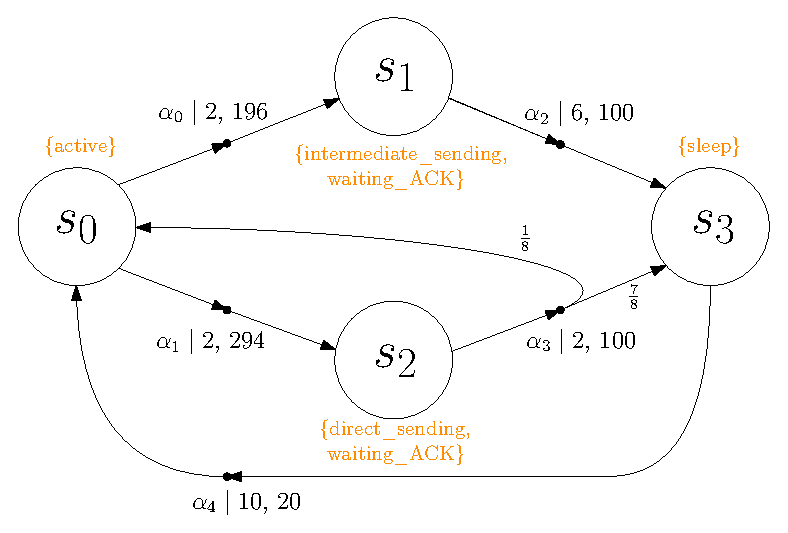
\includegraphics[width=\linewidth]{resources/mdmdp2}
  \end{minipage}
    \captionsetup{justification=centering}
    \caption{Multi-dimensional MDP modelling the situation of Example \ref{main-example}}
    \label{sensornet}
  \end{figure}
  \noindent Consider the following \SSPWE{} problem (covered in Example \ref{sspwe-example}):
  \[
    ?\exists \sigma \; \;  \mathbb{P}^\sigma_{s_0}(\Diamond_{\leq 12} \, \{s_2\}) = 1 \; \wedge \; \mathbb{E}^\sigma_{s_0}(\TS^{\{s_2\}}) \leq 6.
  \]
  Let us re-formulate this problem as a multi-objective Storm-PRCTL query:
  \[
    \mathsf{multi(Pmax>=1\, [F\{``time"\}<=12 } \,``sleep"\mathsf{], \, Rmin=? \, [F }``sleep"\mathsf{])}.
  \]
  \begin{figure}[h!]
  {
  \footnotesize
  \begin{verbatim}
Model checking property
  multi(Pmax>=1 [true Urew{"time"}<=12 "sleep"],
        R[exp]{"time"}min=? [F "sleep"]) ...
Result (for initial states): 5
Time for model checking: 0.049s.
  \end{verbatim}
  }
    \vspace{-2em}
    \caption{Storm-PRCTL query for the \SSPWE{} problem of Example \ref{sspwe-example}}
    \label{sspwe-program}
  \end{figure}
We run Storm by passing the Prism program of Figure \ref{sensornet} as input with this property (cf. Figure \ref{sspwe-program}).
Storm informs us that the result of this query is $5$, what agrees with results of Example \ref{sspwe-example}.
\end{example}

%Finally, we end with an example aggregating the \MOSR{} and \SSPPQ{} problem.
\begin{example}[\textit{\SSPPQ{} problem in Storm}]
Getting back to Example \ref{final-example}, let $\mathcal{M}$ be the MDP of Figure \ref{sensornet}
  Consider the following \SSPPQ{} problem:
  \[
  ?\exists \sigma \;\; \mathbb{P}^{\sigma}_{s_0}(\Diamond_{1: \, \leq 4} \, \{s_3\}) \geq 0.8\; \wedge \;
   \mathbb{P}^{\sigma}_{s_0}(\Diamond_{1: \, \leq 8} \, \{s_3\}) \geq 0.9 \; \wedge \;
  \mathbb{P}_{s_0}^{\sigma}(\Diamond_{2: \, \leq 700} \, \{s_3\}) \geq 0.9.
  \]
  Let us re-formulate this problem as a multi-objective Storm-PRCTL query:
  \begin{itemize}
    \item $\mathsf{\mathcal{Q}_1 : = Pmax=?[F\{``tim
    e"\}<=4
    \,}``sleep"]$,
    \item $\mathsf{\mathcal{Q}_2 := Pmax=? [F\{``time"\}<=8 \,}
  ``sleep"]$,
    \item $\mathsf{\mathcal{Q}_3 := Pmax=? [F\{``energy"\}<=700\,}
  ``sleep"]$,
  \end{itemize}
  \[
    \mathsf{multi(\mathcal{Q}_1, \, \mathcal{Q}_2, \, \mathcal{Q}_3)}.
  \]

We run Storm by passing the Prism program of  Figure  \ref{sensornet} as input with this multi-objective property (cf. Figure \ref{ssppq-program}).
\begin{figure}[h!]
  {
  \footnotesize
  \begin{verbatim}
Model checking property multi(
  Pmax=? [true Urew{"time"}<=4 "sleep"],
  Pmax=? [true Urew{"time"}<=8 "sleep"],
  Pmax=? [true Urew{"energy"}<=700 "sleep"]) ...
Result (for initial states):
Underapproximation of achievable values: Polytope with 5 Halfspaces:
   ( 0.0178571,          1,          0) * x <= 1
   (  0.142857,          1,      0.875) * x <= 1.875
   (         0,          0,          1) * x <= 1
   (         0,          1,          0) * x <= 1
   (         1,          0,          0) * x <= 0.875

Overapproximation of achievable values: Polytope with 6 Halfspaces:
   (         1,          0,          0) * x <= 0.875
   (         0,          1,          0) * x <= 1
   (         0,          0,          1) * x <= 1
   (     0.125,      0.875,          0) * x <= 0.970703
   ( 0.0707965,   0.495575,   0.433628) * x <= 0.929204
   ( 0.0175439,   0.982456,          0) * x <= 0.982456

3 pareto optimal points found (Note that these points are safe, i.e.,
contained in the underapproximation, but there is no guarantee for optimality):
   (     0.875,      0.875,          1 )
   (     0.875,   0.984375,      0.875 )
   (         0,          1,          1 )


Time for model checking: 0.079s.
  \end{verbatim}
  }
    \vspace{-2em}
    \caption{Storm-PRCTL query for the \SSPPQ{} problem of Example \ref{final-example}}
    \label{ssppq-program}
  \end{figure}
The results displayed by Storm are interesting since it gives some informations about how the approximation of the Pareto-curve has been computed.
Indeed, we see that an underapproximation of the curve is computed as well as an overapproximation,
allowing the multi-objective solver to infer an $\epsilon$-(under)-approximation of this curve .
Note that the $\epsilon$ value can be tuned %
%, and that we can plot the Pareto curve for two dimensions cases.with the
with the parameter {\small \color{umons-red}\verb|--multiobjective:precision|}.
Note also that Storm answers \textit{true} to the \SSPPQ{} problem defined above, since $(0.8, 0.9, 0.9)$ is an achievable point of the query, and is situated in a close area between the $\epsilon$-Pareto-optimal points $(0.875, 0.875, 1)$ and $(0.875, 0.984375, 0.875)$.

\end{example}
%and we can plot this $\epsilon$-approximated Pareto curve with the parameter {\small \color{umons-red}\verb|--multiobjective:exportplot|}.

In order to interpret results of multi-objective Storm-PRCTL queries, it would be useful to plot the $\epsilon$-approximated Pareto curve of these queries and visualise it.
In fact, Storm also allows to compute the strategies offering the \textit{Pareto-minimal probabilities}, i.e., the worst achievable points to reach some set of target states in an MDP for a multi-objective context, with a slightly adapted syntax for the probability operator ($
  \mathsf{Pmin=?}
$).
This allows us to determine the set of achievable points under a Pareto-curve.

\begin{example}[\textit{Achievable points for Example \ref{ssppq-example-1}}]
Getting back to Example \ref{ssppq-example-1}, and considering the MDP $\mathcal{M}$ of Figure \ref{sensornet}, we solved the \SSPPQ{} problem
\[
  ?\exists \sigma \;
  \mathbb{P}_{s_0}^\sigma(\Diamond_{1:\leq 4} \,
  \{s_3\}) \geq 0.8 \wedge
  \mathbb{P}_{s_0}^\sigma(\Diamond_{2:\leq 700} \,
  \{s_3\}) \geq 0.9
\]
by considering the pure finite-memory strategy $\sigma^*$ trying once a direct sending and then sending the message via an intermediate node, if the previous sending has failed.
This strategy offers an achievable point $(\frac{7}{8}, 1)$.
We are here interested in plotting the Pareto curve and determining the set of achievable point $U_\mathcal{Q}$ of the following Storm-PRCTL query $\mathcal{Q}$:
\[\mathsf{multi(Pmax = ? [F\{``time"\}<=4}``sleep"\mathsf{], \, Pmax=?[F\{``energy"\}<=700}``sleep"\mathsf{])}
\]
First, we run Storm by passing the Prism program of Figure \ref{sensornet} as well as the Storm-PRCTL query $\mathcal{Q}$.
The result of this query is described in Figure \ref{ssppq-program2}.
\begin{figure}[h!]
  {
  \footnotesize
  \begin{verbatim}
Model checking property multi(
  Pmax=? [true Urew{"time"}<=4 "sleep"],
  Pmax=? [true Urew{"energy"}<=700 "sleep"]) ...
Result (for initial states):
Underapproximation of achievable values: Polytope with 2 Halfspaces:
   (         1,          0) * x <= 0.875
   (         0,          1) * x <= 1

Overapproximation of achievable values: Polytope with 2 Halfspaces:
   (         1,          0) * x <= 0.875
   (         0,          1) * x <= 1

1 pareto optimal points found (Note that these points are safe, i.e.,
contained in the underapproximation, but there is no guarantee for optimality):
   (     0.875,          1 )
  \end{verbatim}
  }
    \vspace{-2em}
    \caption{Storm-PRCTL query for the \SSPPQ{} problem of Example \ref{ssppq-example-1}}
    \label{ssppq-program2}
  \end{figure}
  The under and over approximations of the Pareto curve are the same, that means that the optimal point found is precisely the unique point of the Pareto Curve, i.e., $\mathpzc{P} = \{ (\frac{7}{8}, 1)\}$.
  This optimal point exactly corresponds to the strategy $\sigma^*$.
  Then, in order to determine the worst strategies for this query, we formulate the following Storm-PRCTL query:
  \[\mathsf{multi(Pmin = ? [F\{``time"\}<=4}``sleep"\mathsf{], \, Pmin=?[F\{``energy"\}<=700}``sleep"\mathsf{])}.
  \]
  The result of this query is described in Figure \ref{ssppq-program3}.
\begin{figure}
  {
  \footnotesize
  \begin{verbatim}
Model checking property multi(
  Pmin=? [true Urew{"time"}<=4 "sleep"],
  Pmin=? [true Urew{"energy"}<=700 "sleep"]) ...
Result (for initial states):
Underapproximation of achievable values: Polytope with 3 Halfspaces:
   (        -1,          0) * x <= 0
   (         0,         -1) * x <= -0.875
   ( -0.142857,         -1) * x <= -1

Overapproximation of achievable values: Polytope with 3 Halfspaces:
   (        -1,          0) * x <= 0
   (         0,         -1) * x <= -0.875
   (    -0.125,     -0.875) * x <= -0.875

2 pareto optimal points found (Note that these points are safe, i.e.,
contained in the underapproximation, but there is no guarantee for optimality):
   (     0.875,      0.875 )
   (         0,          1 )
  \end{verbatim}
  }
    \vspace{-2em}
    \captionsetup{justification=centering}
    \caption{Pareto-minimal points for the query describing the problem of Example \ref{ssppq-example-1}}
    \label{ssppq-program3}
  \end{figure}
  The minimal points found for this problem  $(\frac{7}{8}, \frac{7}{8})$ and $(0, 1)$, correspond to the two simple pure memoryless strategies consisting in either always trying a direct sending or just always sending the message via the intermediate node.
  These two points allow us to define lower bounds for achievable points $U_\mathcal{Q}$ (cf. Figure \ref{pareto-2D}).
  \begin{figure}[h!]
    \centering
    \includegraphics[width=0.7\linewidth]{resources/pareto-2D}
  \captionsetup{justification=centering}
  \caption{Pareto curve $\mathpzc{P}$ (in green),
    worst achievable points (in red) and achievable points $U_\mathcal{Q}$ (in blue)}
  \label{pareto-2D}
  \end{figure}
The blue area marks the set of achievable point $U_\mathcal{Q}$ and most of points of this set corresponds to a randomised strategy.
Note that no strategy exist for points in the area under the red dotted line, corresponding to worst achievable points.
\end{example}
